%!TEX root = ../scivis_lbaakman_bvanloon.tex
\chapter{Glyphs} % (fold)
\label{cha:glyphs}
In this chapter a set of \emph{Glyphs} is introduced. Glyphs are a visualization technique which can be used to visualize a vector field by showing its orientation and magnitude. This is done by using icons that show direction and magnitude. A disadvantage of glyphs is the size needed for the icons; as they need to show both direction and magnitude they need to be of some size to convey this information in a clear matter. This means that the number of glyphs used in the visualization needs to be restricted to avoid clutter and glyphs blending together. This means the visualization can not be as `dense' as the scalar visualization, consequently it is not possible to show the information we have for every vertex of the simulation grid. In the next section we discuss how the simulation is sampled and how we prevent cluttering. In \cref{sec:types_of_glyps} the different glyphs we have chosen to implement are discussed.

\section{Method} % (fold)
\label{sec:method}
The main method for constructing glyphs is to sample the dataset and place a glyph at every sample-point. These glyphs are then scaled, colored and rotated based on the the vector and scalar field that are used.

\subsection{Visualization Grid} % (fold)
\label{sub:sampling_grid}
Since glyphs can not be shown for every vertex of the simulation due to their size, we need to subsample the simulation. The number of sampling points denotes how many glyphs are shown. Fewer sampling points result in fewer glyphs and thus less clutter, but also less displayed information. Increasing the number of sampling points increases the amount of information shown, but is also likely to increase cluttering which can interfere with how well the information can be understood by the user. 

To facilitate the sampling, a visualization grid is constructed\footnote{Note that the visualization grid is also used in combination with other visualization methods, but since the glyph visualization is the first technique in which the grid is used, it is introduced in this chapter.}. This grid is defined on top of the simulation grid, ensuring that simulation is covered. Each vertex of the visualization grid is contained within some cell of the simulation grid. When data is requested from vertices in the visualization grid the values at that vertex are calculated using bilinear interpolation of the vertices of its containing cell in the simulation cell. 

Given a cell $C$ with four vertices: the upper left vertex $(C_{UL})$, the upper right vertex $(C_{UR})$, the lower left vertex $(C_{BL})$ and the lower right vertex $(C_{BR})$, a scalar value at some position $p = (p_x, p_y)$ within the cell is bilinear interpolated according to:
\begin{align*}
	s & = C_{UL} * (1 - p_x ) * (1 - p_y) \\
		& +	C_{UR} *  p_x  * (1 - p_y) \\
		& +	C_{BL} *  (1 - p_x ) * p_y \\
		& +	C_{BR} *  p_x  * p_y. \\
\end{align*}
Note that the the position $p$ is normalized within the cell, \ie $p_x,\, p_y \in [0, 1]$. Vectors are interpolated by bilinear interpolation of their components. Since it is unlikely to find inflection points between the sampled points of our vector fields this is sufficient, as long as we use a grid with a reasonable high sampling density.

\subsubsection{Jitter} % (fold)
\label{ssub:jitter}
When glyphs are shown on an uniform grid, beating artifacts might appear. These patterns can be avoided by adding some random shifts in the sampling grid. This is done by translating each vertex of the visualization grid with some random values. These absolute values of these translations in both the x and y direction is always smaller than the size of cell, to ensure that the topological ordering of the grid stays the same. The translation in the x direction is determined independent of the translation in the y direction. To determine the translation in some direction a value is sampled from a uniform distribution, with the previous indicated range, the resulting offset is scaled with the jitter factor. This allows us to control how much the grid is jittered.  If the jitter factor is zero, the jittered grid reduces to an uniform grid. \Cref{fig:jitter} illustrates the effect of adding jitter, the visualization that uses a grid without jitter in \cref{fig:jitter:nojitter} contains beating artifacts, while \cref{fig:jitter:jitter} does not.
\begin{figure}[tbh]
	\centering
	\begin{subfigure}{0.45\textwidth}
		\centering
		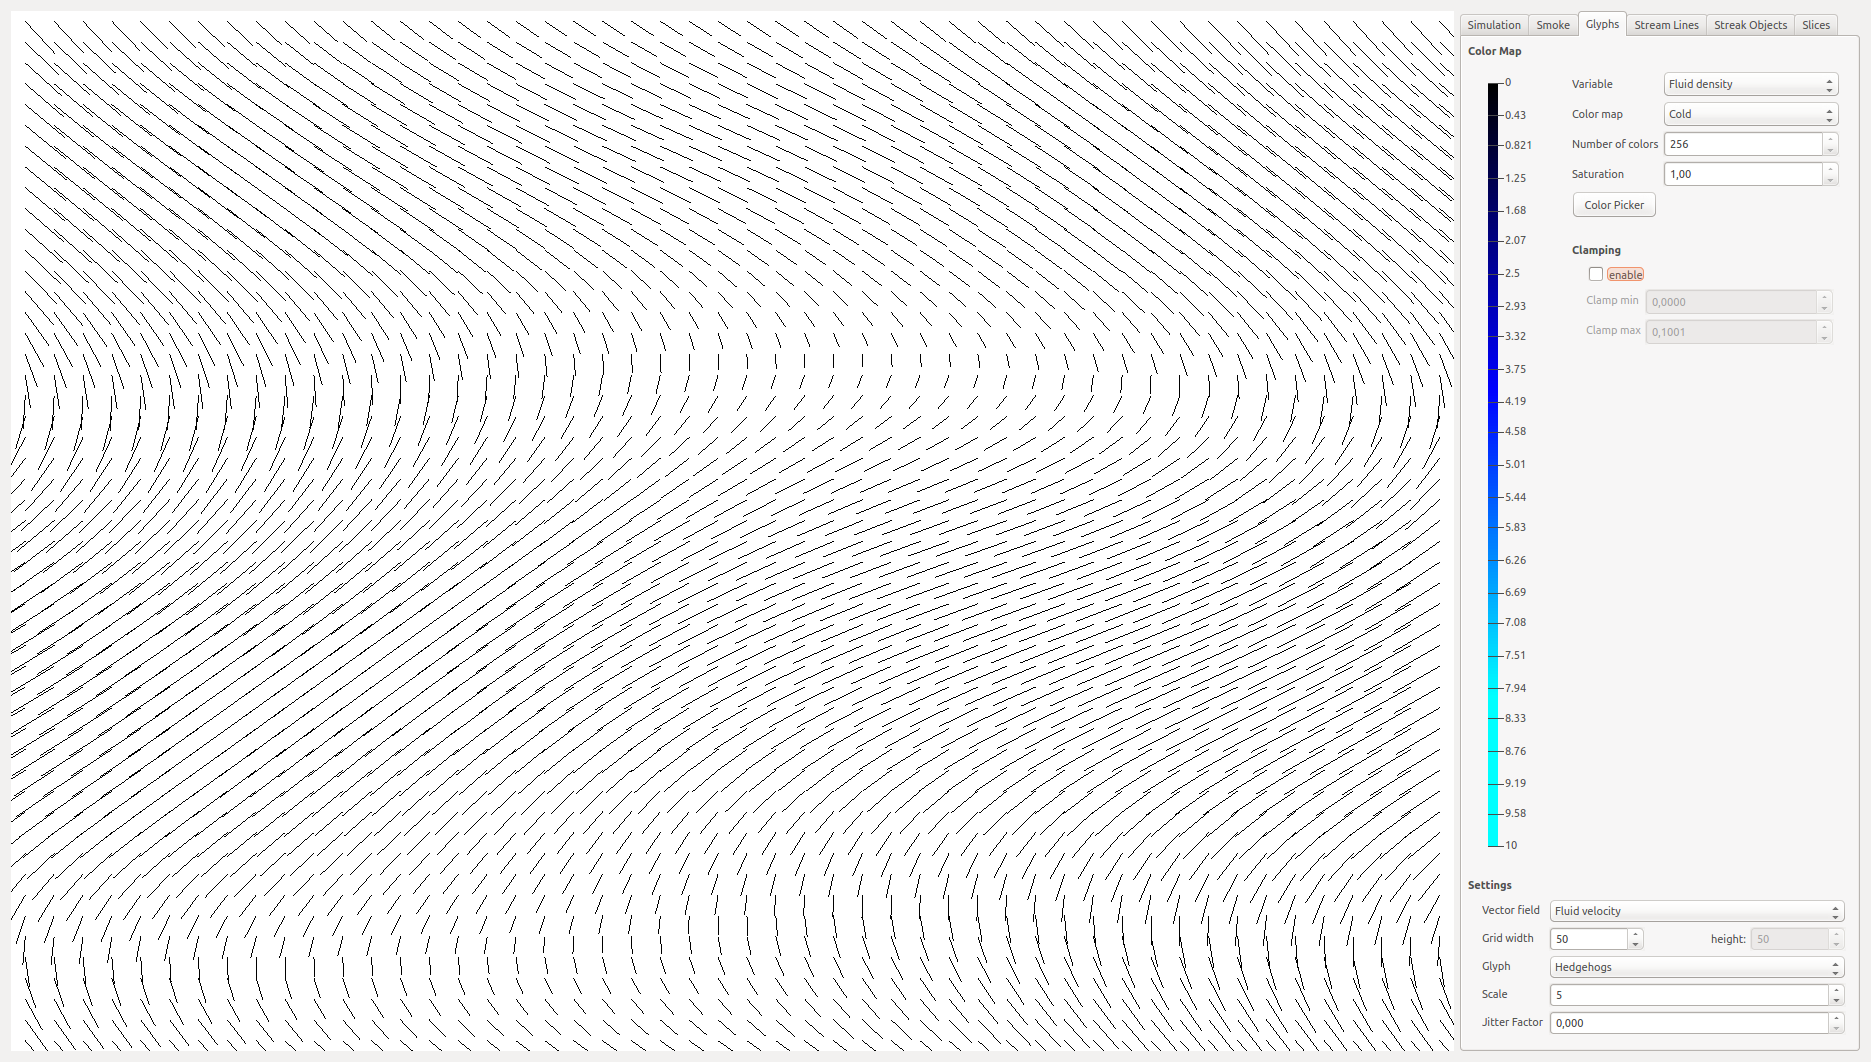
\includegraphics[width=0.9\textwidth, trim={35px 30px 430px 30px}, clip]{img/glyphs/nojitter}
		\caption{No jitter}
		\label{fig:jitter:nojitter}
	\end{subfigure}
	\hspace{30px}
	\begin{subfigure}{0.45\textwidth}	
		\centering
		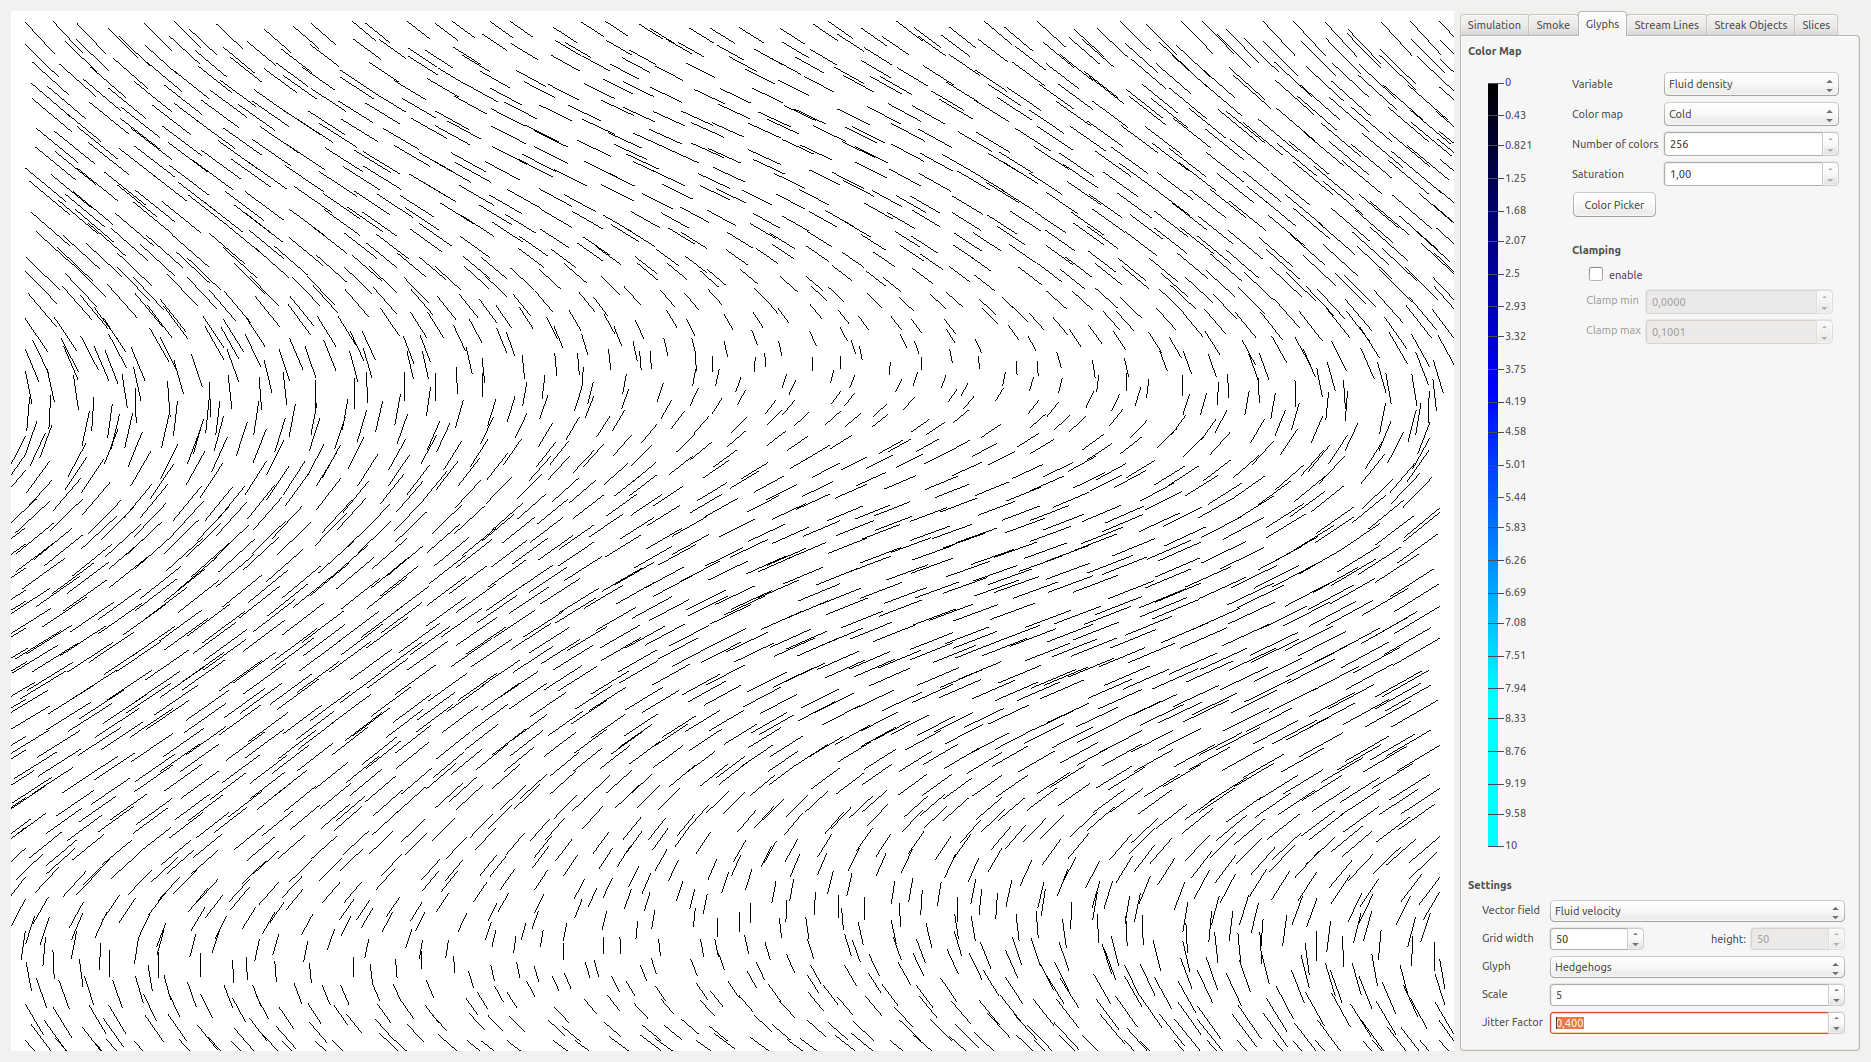
\includegraphics[width=0.9\textwidth, trim={35px 30px 430px 30px}, clip]{img/glyphs/jitter_0.4}
		\caption{Jitter factor = 0.4.}
		\label{fig:jitter:jitter}
	\end{subfigure}
	\caption{The visualization of a vector field using glyphs \subref{fig:jitter:nojitter} without and \subref{fig:jitter:jitter} with jittering.}
	\label{fig:jitter}
\end{figure}

\subsection{Scaling} % (fold)
\label{sub:scaling}
Glyphs are scaled to show the magnitude of the vector. In our application the size of the glyph is scaled relative to the size of its containing cell. This is done to prevent glyphs from becoming too large which causes cluttering, another advantage is that glyphs will take up more space when the cell size increases, making optimal use of the available space. To ensure the scaling of the glyphs is linear glyphs have no minimum size. This has as disadvantage that glyphs of vectors with a very small magnitude might not be visible, but makes for a more naturally ordered magnitude. The scaling can also be tweaked using a scale-factor which can be set by the user.
\begin{figure}[tbh]
	\centering
	\begin{subfigure}{0.45\textwidth}
		\centering
		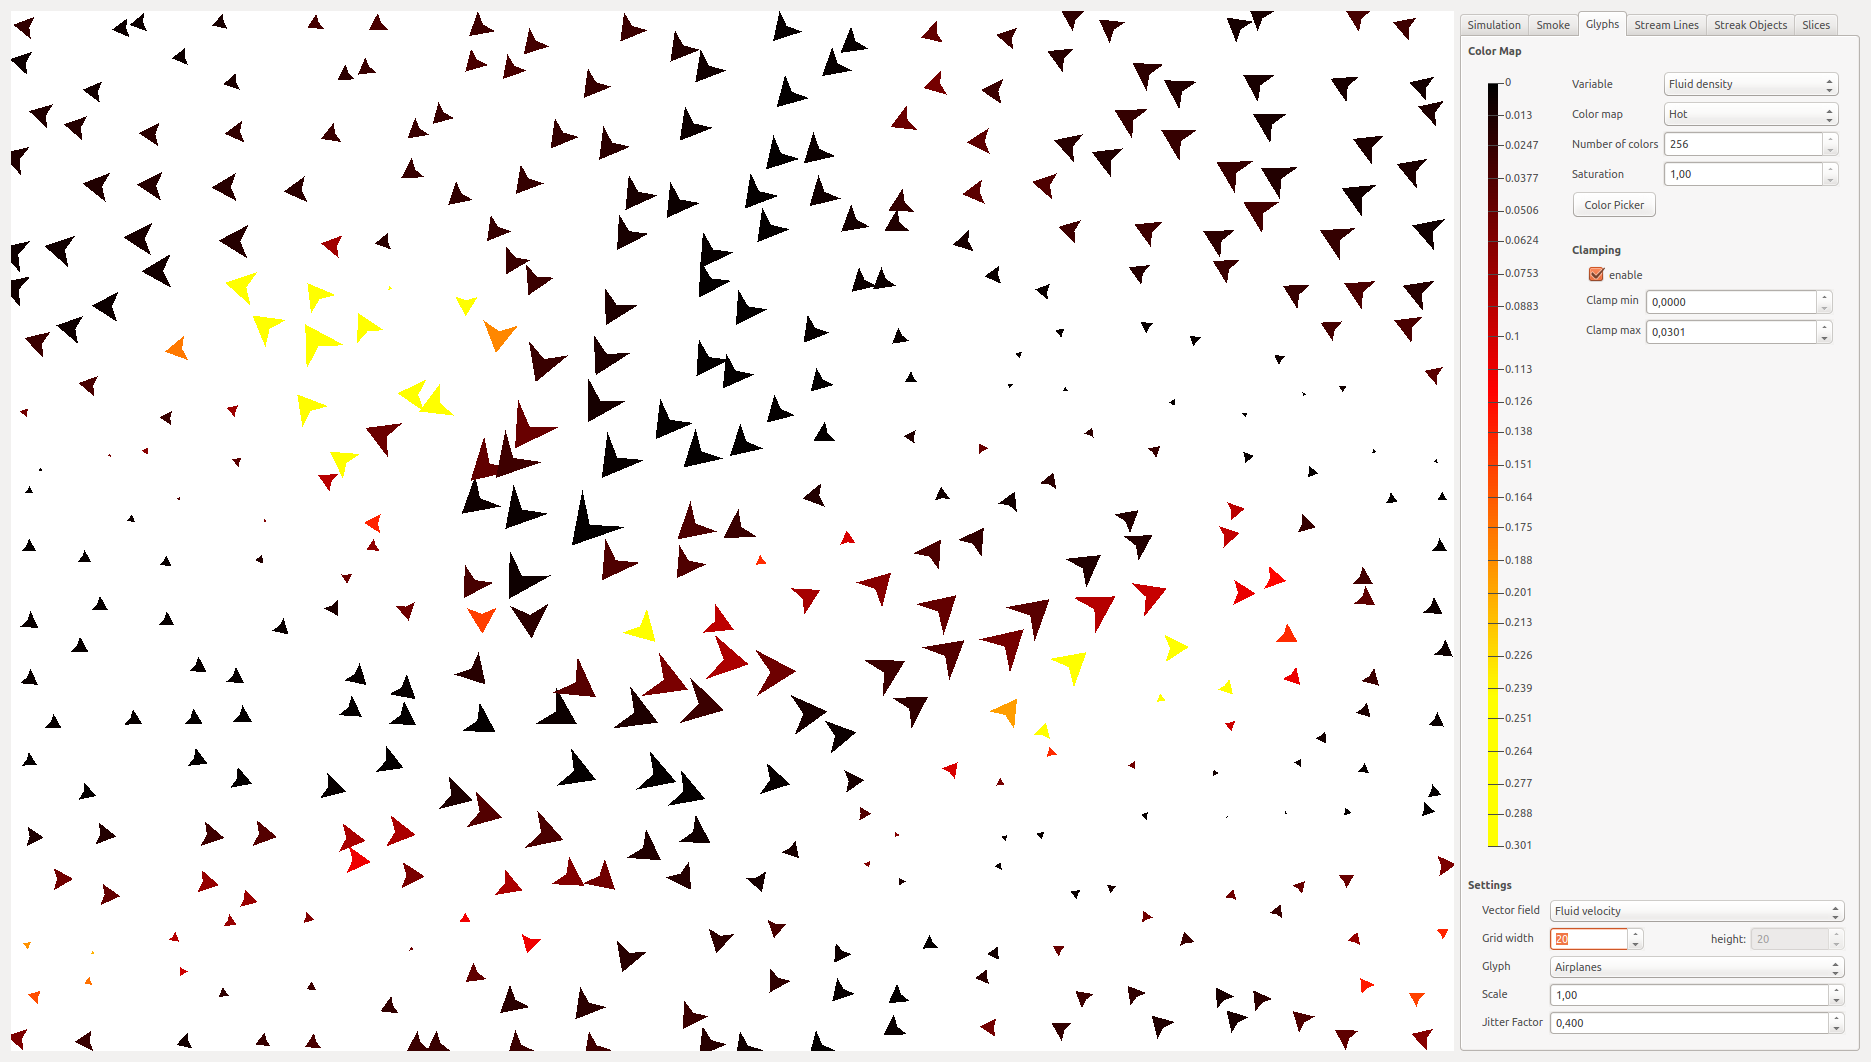
\includegraphics[width=0.9\textwidth, trim={35px 30px 430px 30px}, clip]{img/glyphs/scaling_20}
		\caption{Airplane glyphs on a 20x20 grid.}
		\label{fig:scaling:20}
	\end{subfigure}
	\hspace{30px}
	\begin{subfigure}{0.45\textwidth}	
		\centering
		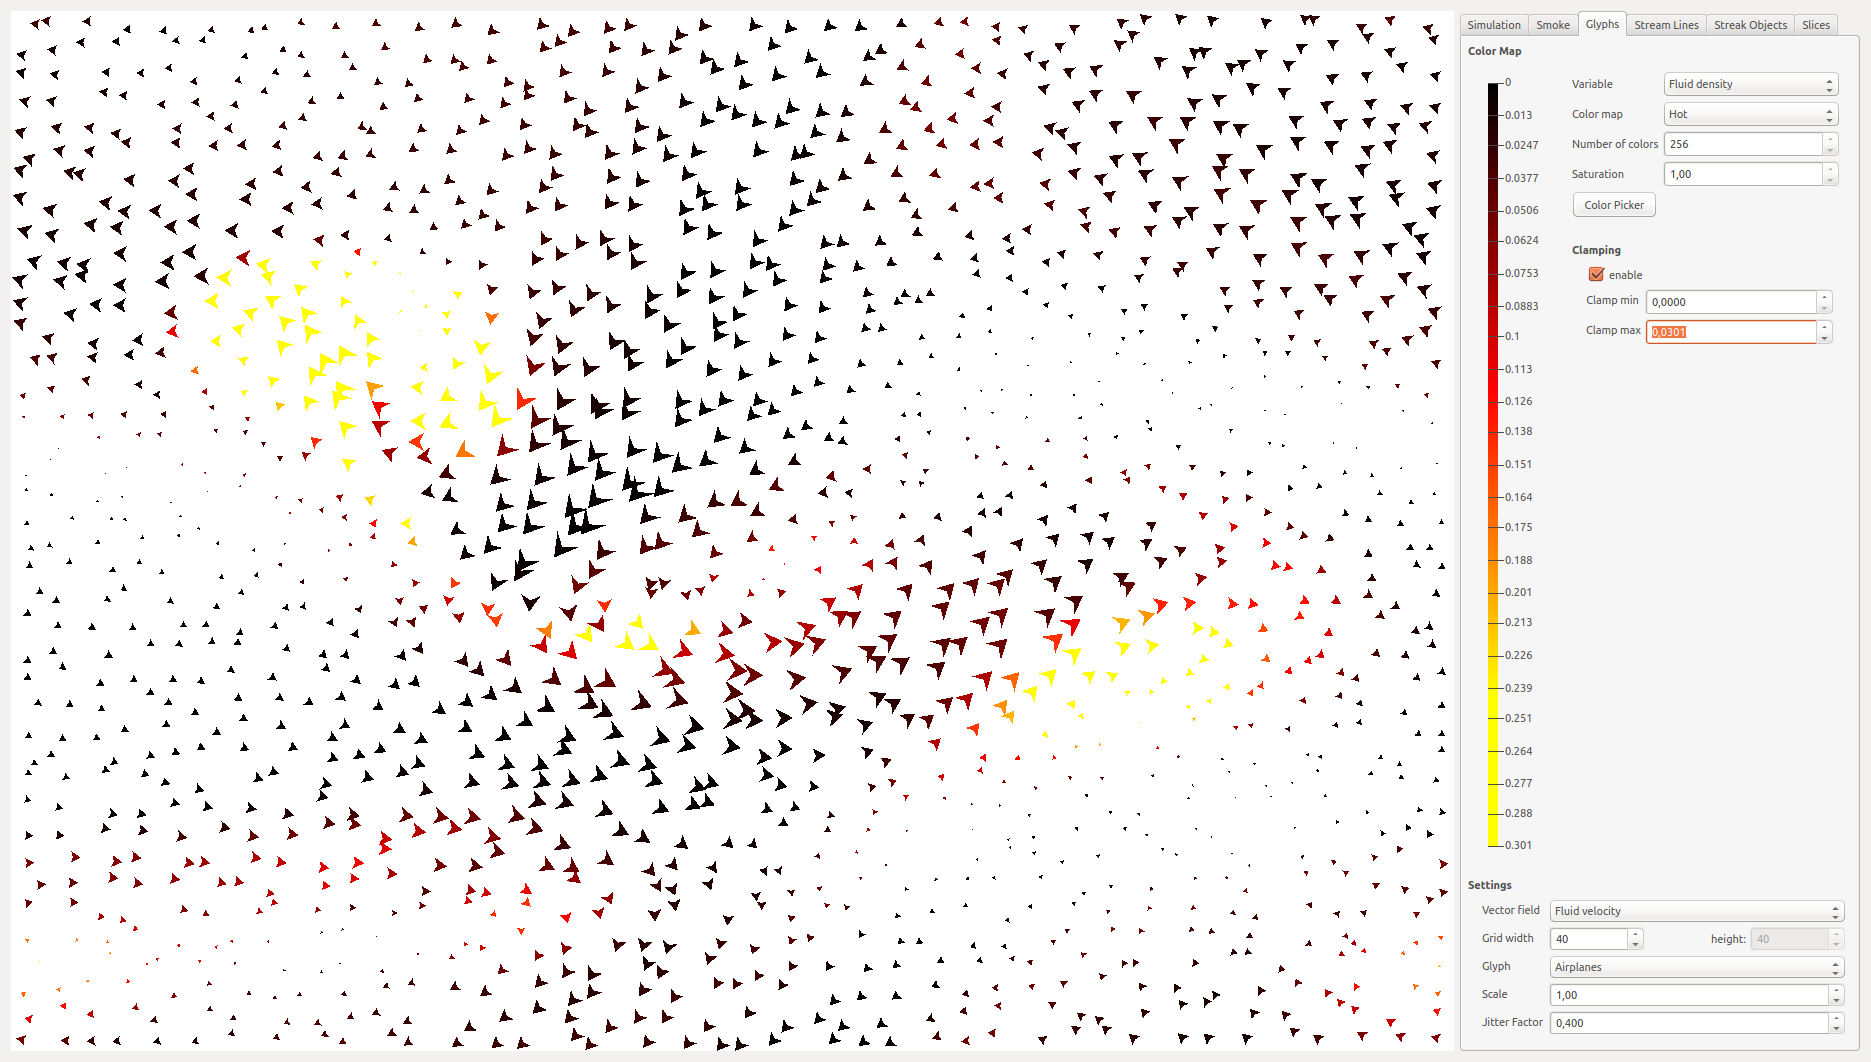
\includegraphics[width=0.9\textwidth, trim={35px 30px 430px 30px}, clip]{img/glyphs/scaling_40}
		\caption{Airplane glyphs on a 40x40 grid.}
		\label{fig:scaling:40}
	\end{subfigure}
	\caption{In this figure the same simulation is shown twice using airplane glyphs on \subref{fig:scaling:20} a $20 \times 20$ and \subref{fig:scaling:40} a $40 \times 40$ grid.}
	\label{fig:scaling}
\end{figure}

% section method (end)



\section{Types of Glyps} % (fold)
\label{sec:types_of_glyps}
This section introduces the different glyphs we support. 

\subsection{Hedgehogs} % (fold)
\label{sub:hedgehogs}
The simplest form of glyphs are hedgehogs. Hedgehogs are lines which are placed in the direction of the vector and stretched relative to the magnitude of the vector they represent. The glyph can be colored in two ways, first we can let the color of the glyph correspond with the vector magnitude. This way the magnitude is conveyed to the user by both the length and the color of the glyph which can help inverse mapping. Alternatively the glyph can be colored according to some scalar value. This increases the information density of the visualization, but might reduce the clarity of the visualization.

Hedgehogs have as an advantage that the glyphs take up relatively little space. A major drawback of hedgehogs is that it is not possible to distinguish two vectors going in opposite directions, as they are be represented by the same line. 

\subsection{Triangles} % (fold)
\label{sub:triangles}
The triangle glyph is one of the simplest glyphs that can give directional information. It is constructed by placing the middle of one side of the triangle orthogonal on the vector. The two others sides are stretched in the direction of the vector relative to the vectors magnitude. Thus, the triangle will appear longer as the magnitude of the vector increases. This also increase the area of the triangle, which makes the glyphs representing vectors with a greater magnitude more prominent.

Although triangles properly convey the direction in most cases, a problem arises when the magnitude scales the triangles such that the extended sides become as long as the base side.  When this happens the triangle becomes equilateral and can no longer be mapped to a single direction. This could be solved by curving the two extended sides inwards or by making the triangle into an arrow.

The triangle glyph is implemented such that the base side has a fixed length. This has as side-effect that vectors with a small magnitude might appear as lines orthogonal to the vector field. This can confuse users not aware of this effect, who therefore might interpret the triangle as a hedgehog. This increases the learning curve of the visualization. A solution to this problem would be to scale the base of the triangle with the magnitude of the vector. 

\subsection{Airplanes} % (fold)
\label{sub:airplanes}
In the previous section two flaws of the triangle where pointed out that could cause possible difficulty with the inverse mapping process. These flaws are fixed by the airplane glyph discussed in this section. The airplane glyph is a 3D glyph that is defined as two mirrored triangles joined at one side forming an airplane like structure. Depending on the vector magnitude the sides joined together will be pulled upwards, while the free vertex of both triangles will be pulled backwards. This has as effect that the airplane will become longer and pointier as the magnitude increases. Therefore the larger the magnitude becomes, the more prominent the direction of the glyph will be. This has two positive effects. Increasing magnitudes will have a clear natural order and as the magnitude increases the direction of the glyph becomes better visible. Since one can argue that the direction of a vector is of more importance when its magnitude increases this can be seen as a positive effect.

Since the airplane is a 3D glyph it is possible to use shading with the glyph visualization. This means that in the case of overlapping glyphs, single glyphs can be distinguished more easily due to the visual clues shading offers. 

The airplane glyph has a drawback concerning its scaling. When an airplane glyph is scaled up based on some magnitude, its wings are pushed down and its base is pulled up. Because the perspective in which the glyphs are shown (top-down) is not orthogonal to the glyphs surface, the `wings' of the glyph become skewed, meaning that the visible surface of a glyph is smaller than its real surface. This effects increases as the glyph is scaled up, meaning that its relative surface becomes smaller as its corresponding magnitude increases which means the ordering of the magnitude becomes non-linear. 
% subsection airplanes (end)


\subsection{Results} % (fold)
\label{ssec:glyphs:results}
This section presents and discusses three visualizations of the same vector field with different glyphs.

\begin{figure}[tb]
	\centering
	\begin{subfigure}{0.6\textwidth}
	\centering
	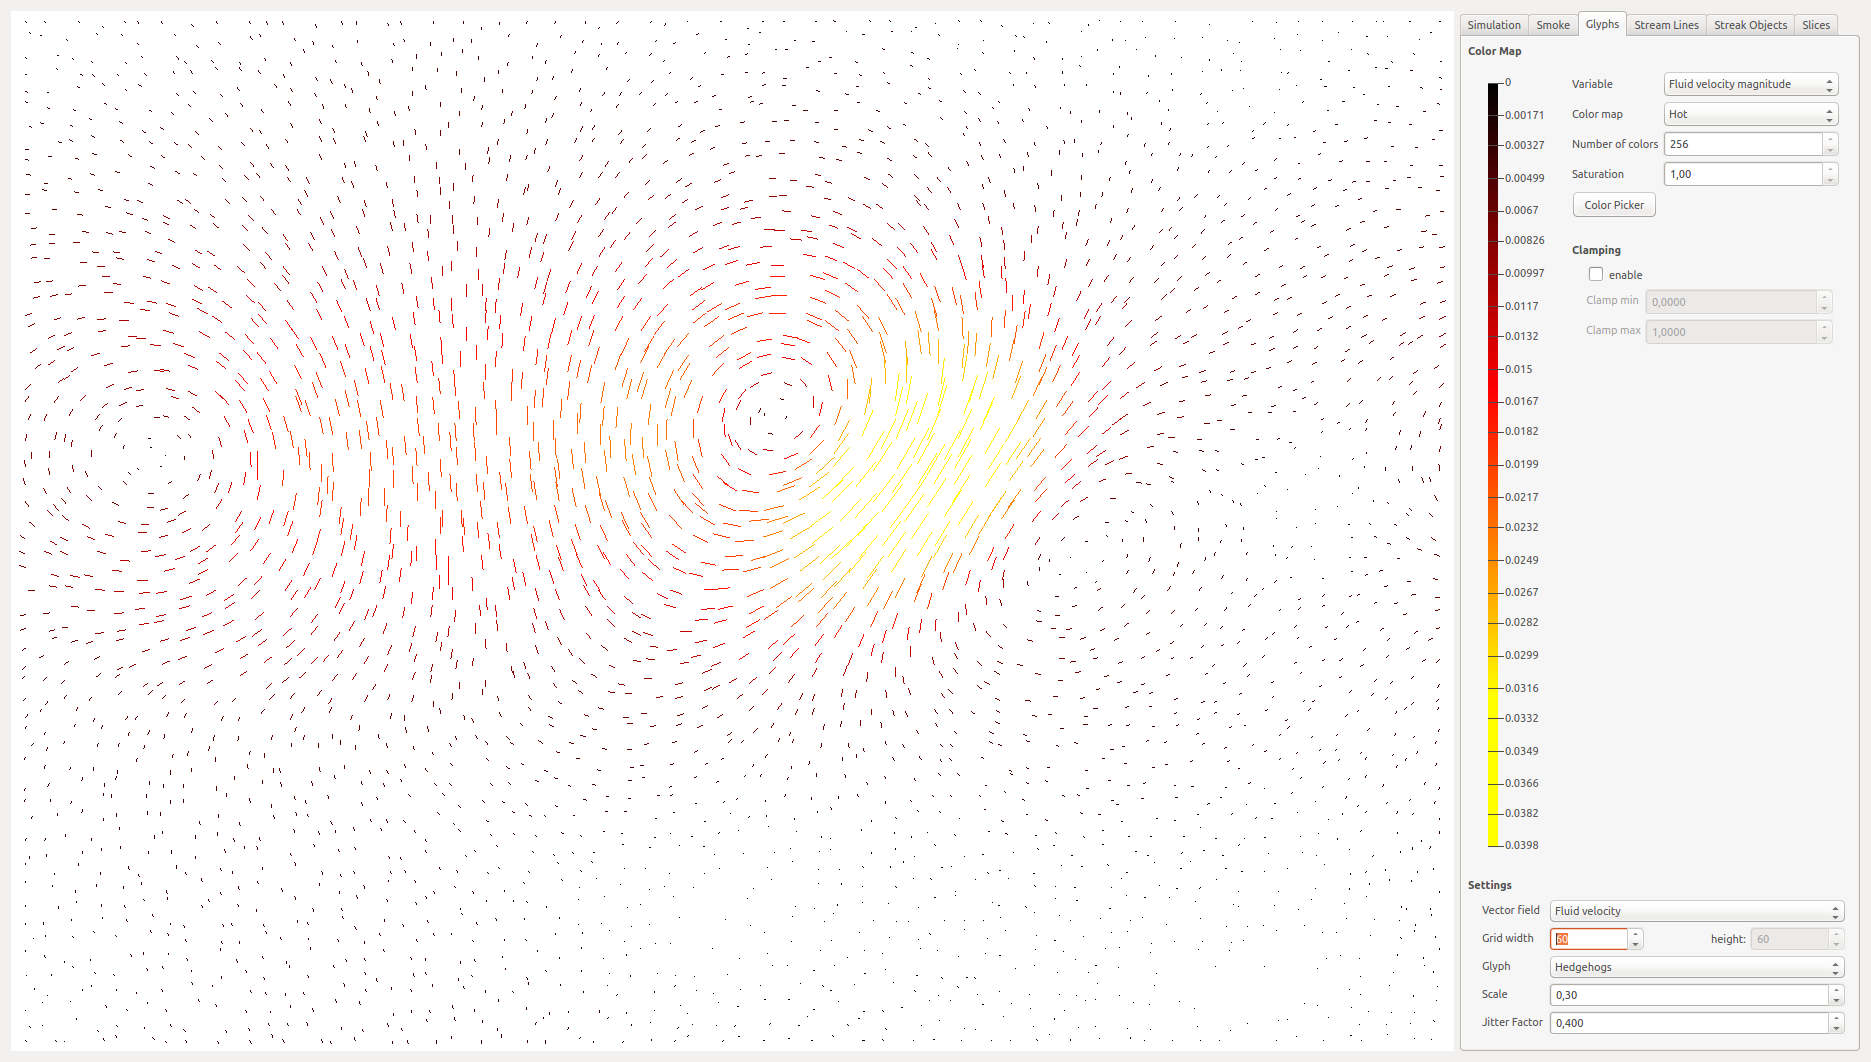
\includegraphics[width=\textwidth, trim={35px 30px 430px 30px},clip]{img/glyphs/hedgehogs.png}
	\caption{Hedgehogs on a 60x60 grid.}
	\label{fig:glyphs:hedgehogs}
	\end{subfigure}
	\begin{subfigure}{0.6\textwidth}
		\centering
		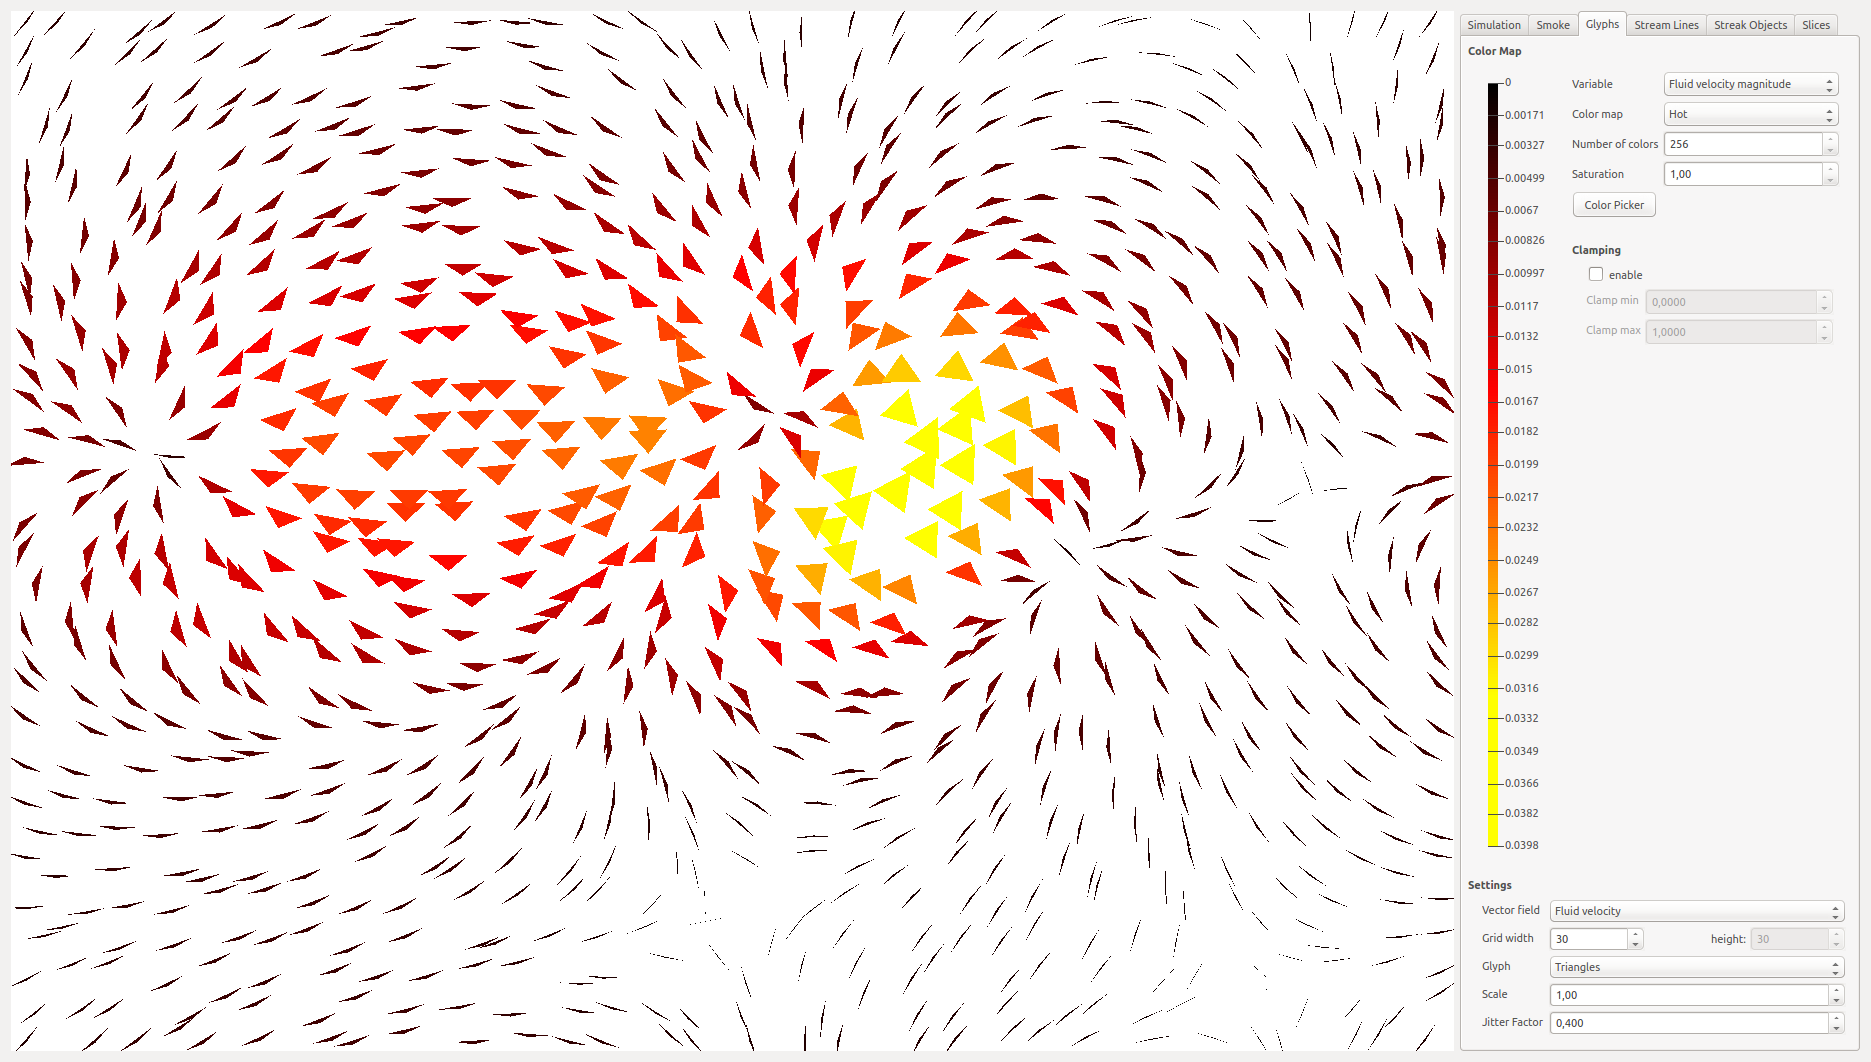
\includegraphics[width=\textwidth, trim={35px 30px 430px 30px},clip]{img/glyphs/triangles.png}
		\caption{Triangles on a 30x30 grid.}
		\label{fig:glyphs:triangles}
	\end{subfigure}
	\begin{subfigure}{0.6\textwidth}
		\centering
		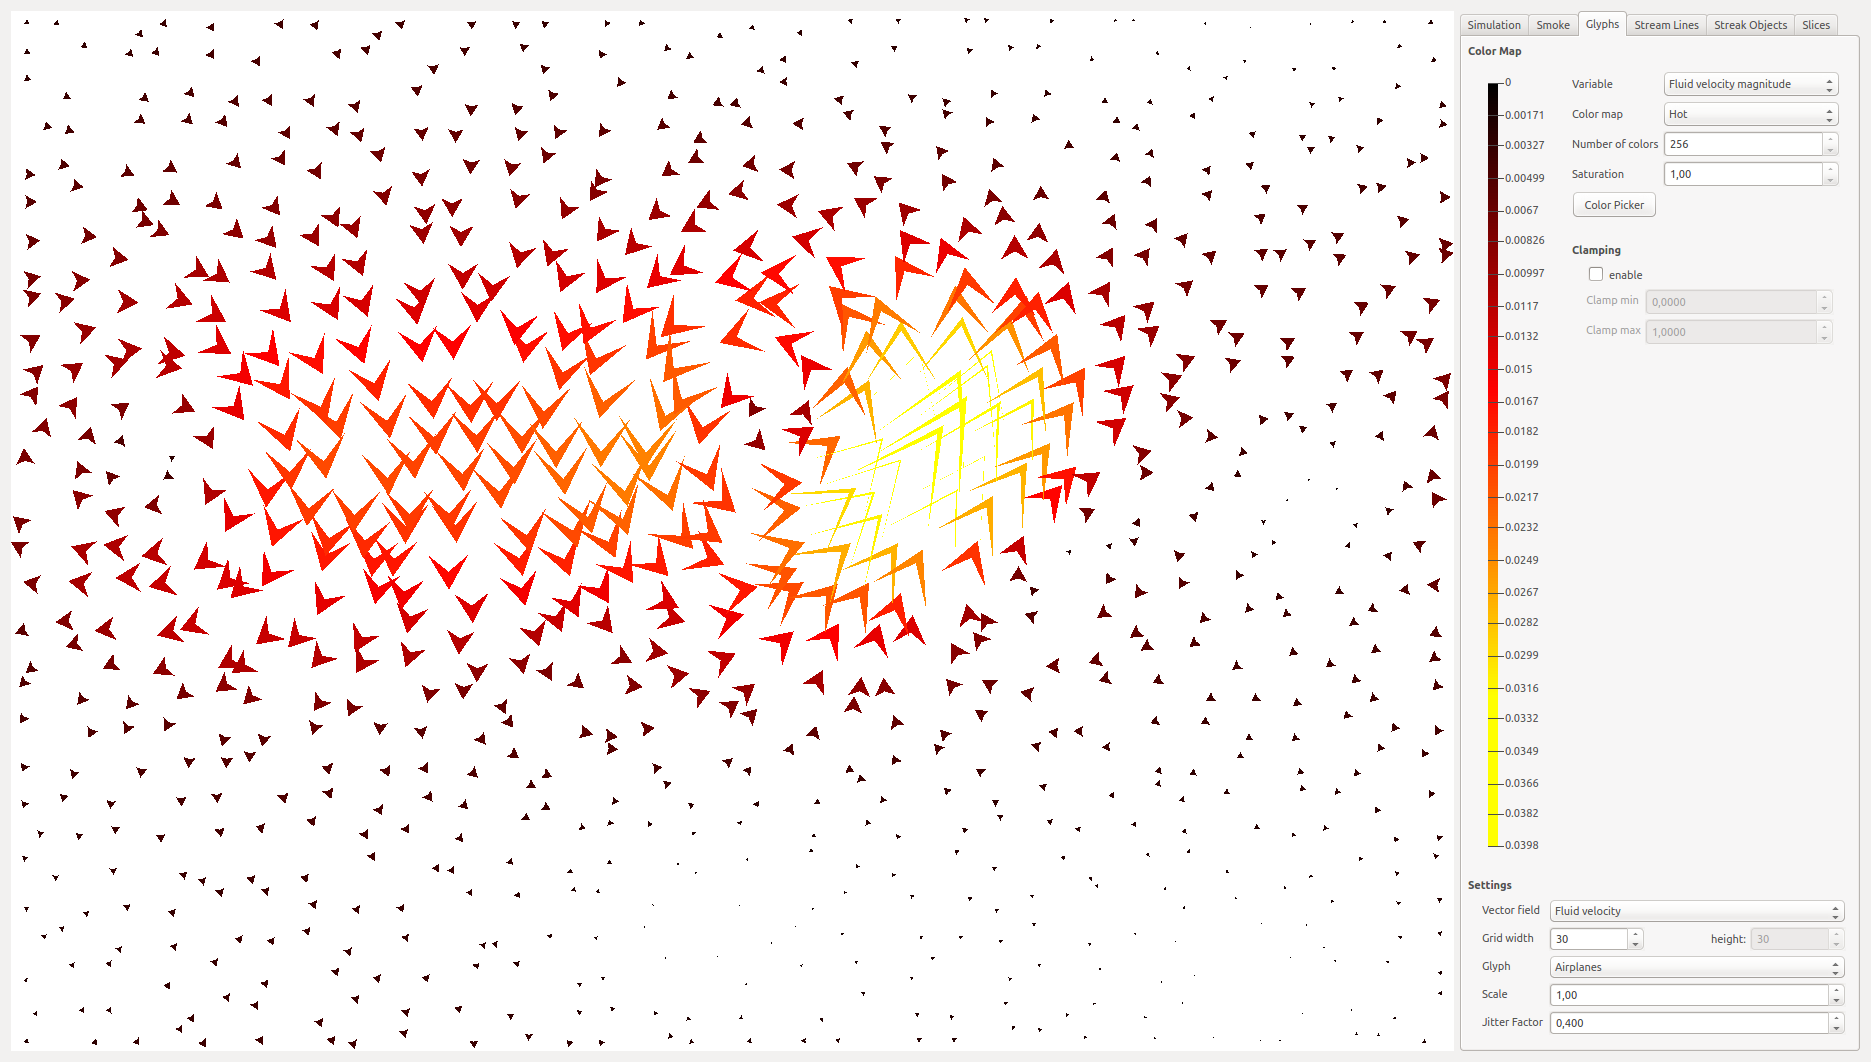
\includegraphics[width=\textwidth, trim={35px 30px 430px 30px},clip]{img/glyphs/airplanes.png}
		\caption{Airplanes on a 30x30 grid.}
		\label{fig:glyphs:airplanes}
	\end{subfigure}
	\caption{Three visualizations of the same vector field, \velocity, \subref{fig:glyphs:hedgehogs} hedgehogs \subref{fig:glyphs:triangles} triangles, and \subref{fig:glyphs:airplanes} airplane glyphs.}
	\label{fig:glyphs}
\end{figure}

Observing \cref{fig:glyphs} we can make the following observations. Firstly the hedgehog glyphs in \cref{fig:glyphs:hedgehogs} show the general flow of the vector field. A disadvantage of this visualization is that it is hard to see the size of an individual hedgehog, making it harder to use its magnitude for the inverse mapping to the fluid velocity. Furthermore is it not possible to distinguish sources and sinks since the glyphs do not have a clear origin and destination. Contrary to the hedgehogs the triangle glyphs illustrate the direction of the vector field. We can also see see the magnitude of the vector represented by the glyphs. The disadvantages of these glyphs we mentioned earlier are also visible: when the magnitude of the glyph is near zero the triangles appear as lines and when its magnitude is around its max the triangle becomes nearly equilateral making it harder to see the direction in which they are pointing. Finally the airplane glyphs indicate both direction and magnitude, but are put a greater emphasis on the direction of glyphs with a larger magnitude. The discussed disadvantages are also illustrated by \cref{fig:glyphs:airplanes}, as glyphs representing vectors with a large magnitude are some strange `v' that is hard to observe.

In general we conclude that although glyphs provide a nice way to visualize vector data this method also has many problems. The glyphs require space to be drawn, can occlude each other, sampling artifacts can appear, and directions are sometimes hard to decode. Some of these problems are partly solved by adding jitter to the grid and by using different types of glyphs, but most of these problems cannot be solved completely.

% section results (end)
